\section{Introduction}




%Retrieval-Augmented Generation (RAG) systems~\cite{lewis2020retrieval, gao2023retrieval} have garnered significant attention recently due to their ability to generate informative and coherent responses by leveraging external knowledge sources. 

Retrieval-Augmented Generation (RAG) systems~\cite{lewis2020retrieval, gao2023retrieval} enhance Large Language Models (LLMs) by incorporating external knowledge bases, enabling more precise and contextually relevant responses~\cite{gao2023retrieval, yu2024evaluation, huang2024survey}. As these systems become integral to a variety of applications~\cite{zakka2024almanac, asai2023retrieval, guo2023retrieval},
it's imperative to develop robust and comprehensive evaluation frameworks to assess their performance and identify areas for improvement.
%As RAG becomes increasingly prevalent in various applications, developing robust and comprehensive evaluation frameworks to assess their performance and identify areas for improvement is crucial.
Evaluating RAG systems, however, presents several challenges:

(1) \emph{modular complexity}: The modular nature of RAG systems, comprising both a retriever and a generator, complicates the design of effective evaluation metrics. It is crucial to establish metrics that can holistically assess the entire system as well as evaluate the individual modules and their interplay~\cite{yu2024evaluation}, allowing for fully understanding the sources of the errors and misses and how they are generated.
% allowing for fully understanding the strengths and weaknesses of each component and how they work together within the system.
(2) \emph{metric limitation}: 
Existing metrics for evaluating RAG systems, which are often rule-based or coarse-grained, fall short in providing accurate and interpretable results. Specifically, traditional metrics like recall@k and MRR~\cite{voorhees1999trec} for retrievers depend on annotated chunks and a rigid chunking approach, missing out on the full semantic scope of the knowledge base. For generators, typical measures such as n-gram-based (e.g., BLEU~\cite{papineni-etal-2002-bleu}, ROUGE~\cite{lin-2004-rouge}), embedding-based (e.g., BERTScore~\cite{zhang2019bertscore}), and LLM-based methods~\cite{wang2024evaluating} perform well with concise answers but fail to detect finer distinctions in longer responses. To bridge these gaps, it is essential to develop detailed, semantic-based evaluation metrics that effectively capture the intricacies and overall quality of both the retrieval and generation components in RAG systems.
%existing metrics for evaluating RAG systems are often limited to rule-based or coarse-grained approaches, leading to inaccurate and hard-to-interpret results. For the retriever, the standard evaluation involves chunk-level recall or ranking metrics such as recall@k and MRR~\cite{xx}. However, these metrics require annotated ground truth chunks and restrict the RAG to use a fixed chunking strategy. Moreover, they fail to capture the semantic relevance of the retrieved chunks, as the relevant chunks in the knowledge base are not limited to the annotated ones. For the generator, previous works typically assess the response-level similarity between the generated response and the ground truth answers using methods such as n-gram based (e.g., BLEU~\cite{papineni-etal-2002-bleu}, ROUGE~\cite{lin-2004-rouge}), embedding-based (e.g., BERTScore~\cite{zhang2019bertscore}), and LLM-based evaluators~\cite{wang2024evaluating}. While these methods are effective for extractive question answering tasks with short ground truth answers, they struggle to identify subtle differences between the response and ground truth in long-form answers. To overcome these limitations, there is a need for fine-grained, semantic evaluation metrics that can capture the nuances and quality of both the retriever and generator components.
(3) \emph{metric reliability}: 
%the third challenge is Metric Reliability. 
the reliability of existing metrics for RAG remains under-explored. Effective evaluation metrics must not only accurately reflect system performance but also align with human judgments to ensure their utility in real-world scenarios.
%the reliability of the metrics used for evaluating RAG systems is an untouched problem. Ensuring that the metrics accurately reflect the system's performance and correlate with human judgments is crucial for effective evaluation.

% To address these limitations, we propose \benchname, a novel evaluation framework that offers fine-grained evaluation for both retrieval and generation. Built upon RefChecker~\cite{hu2024refchecker}, a claim-level hallucination detection framework, \benchname introduces holistic metrics by organizing the checking results of RefChecker. \benchname takes the user query, retrieved context, response, and ground truth answer as input and outputs 
% (i) overall metrics: claim-level precision, recall, and F1 score;
% (ii) retrieval metrics: claim recall and context precision;
% (iii) generator metrics: context utilization, noise sensitivity, hallucination, self-knowledge, and faithfulness. 

% To overcome these challenges, we introduce \benchname, an innovative evaluation framework designed for detailed analysis of both retrieval and generation processes. Building on the foundation of RefChecker~\cite{hu2024refchecker}, a claim-level hallucination detection framework, \benchname\space enhances evaluation by integrating RefChecker's results into comprehensive metrics that are specially designed for RAG. \benchname\space processes the user query, retrieved context, response, and ground truth answer, producing a suite of metrics:

To overcome these challenges, we introduce \benchname, an innovative evaluation framework designed for detailed analysis of both retrieval and generation processes. \benchname\space is based on claim-level entailment checking which involves operations of extracting claims from the response and ground truth answer and checking them against other texts. This approach enables fine-grained evaluation instead of response-level assessment. \benchname\space processes the user query, retrieved context, response, and ground truth answer, producing a suite of metrics:

\begin{enumerate*}
    % \item \textbf{Overall Metrics}: Claim-level precision, recall, and F1 score, which provide a holistic view of system performance at the claim level.
    % \item \textbf{Retrieval Metrics}: Claim recall and context precision, which aim to evaluate the retrieval component's effectiveness.
    % \item \textbf{Generation Metrics}: Context utilization, noise sensitivity, hallucination, self-knowledge, and faithfulness, which collectively provide interpretable evaluation aspects.
    \item \textbf{Overall Metrics} to provide a holistic view of the system performance, assessing the overall quality of the generated responses.
    \item \textbf{Diagnostic Retriever Metrics} to evaluate the effectiveness of the retriever, identifying its strengths and weaknesses in finding relevant information from the knowledge base.
    \item \textbf{Diagnostic Generator Metrics} to assess the performance of the generator, diagnosing how well the generator utilizes the retrieved context, handles noisy information, and generates accurate and faithful responses.



    
\end{enumerate*}




% \begin{figure}
%     \centering
%     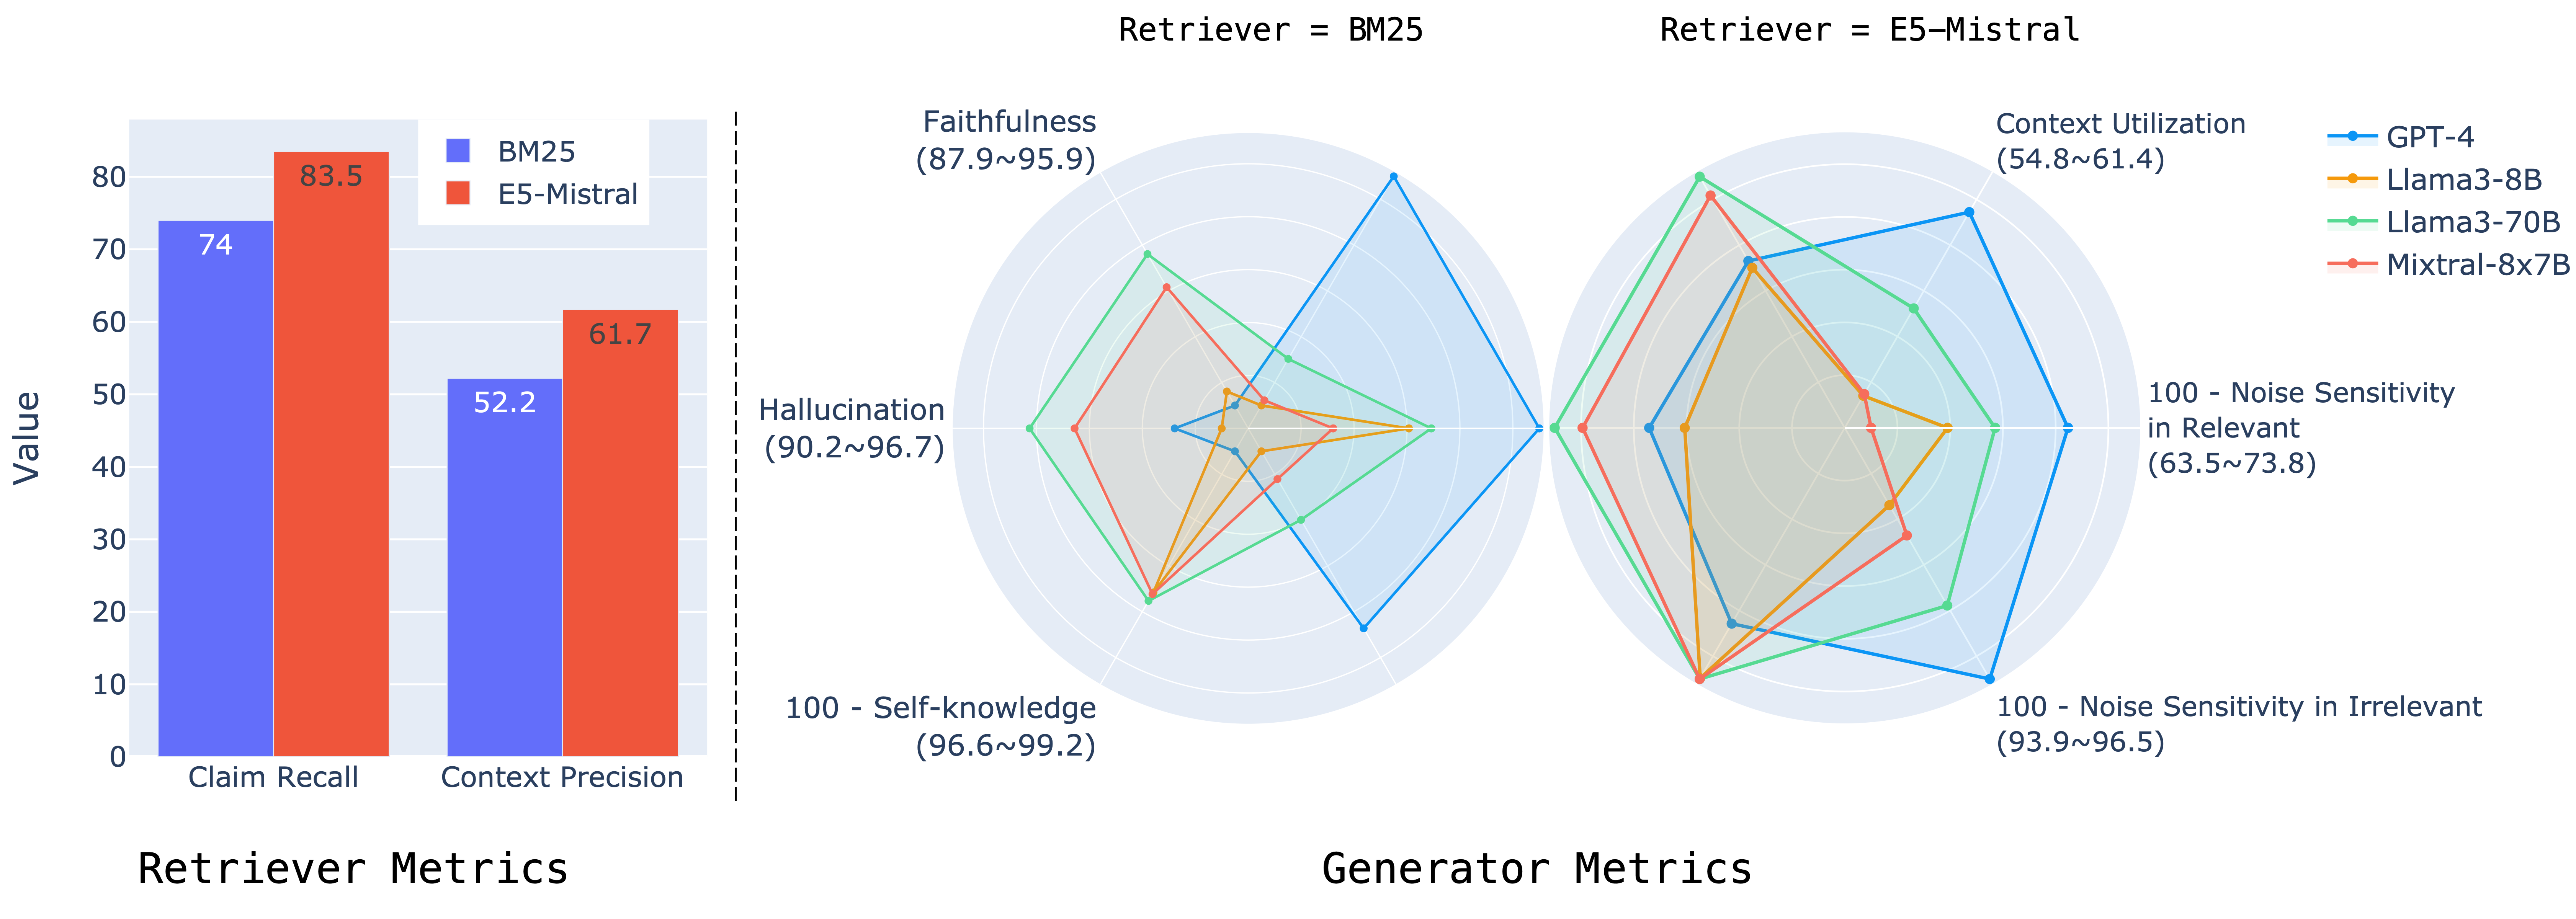
\includegraphics[width=0.9\textwidth]{figures/intro_radar.png}
%     \caption{Results of the metrics for evaluated 8 RAG systems (2 retrievers and 4 generators) on our benchmark datasets averaged over 10 domains. From the radar chats, it is evident that, with the help of \benchname, we can see how improvements in retriever performance (from BM25 to E5-Mistral) lead to enhanced metrics across different generators, providing a clear and intuitive understanding of the system's efficacy.}
%     \label{fig:intro_metrics}
% \end{figure}

% Fig.~\ref{fig:intro_metrics} shows the results for metrics of retriever and generator on our benchmark. 
Compared to existing evaluation frameworks, \benchname\space provides a more comprehensive assessment of RAG systems. While some frameworks offer fine-grained evaluation only on certain metrics (e.g., RAGAS~\cite{es2023ragas}, TruLens~\cite{TruLens}, ARES~\cite{saadfalcon2023ares}) or evaluate specific aspects of RAG (e.g., RGB~\cite{chen2024benchmarking}, RECALL~\cite{liu2023recall}, NoMIRACL~\cite{thakur2023nomiracl}), \benchname's metrics are all based on fine-grained claim-level checking and are designed to provide actionable insights into the sources of errors. 

To ensure the reliability of \benchname, we annotate a human judgment dataset to assess the correlations between the proposed metrics and human judgments. This meta-evaluation validates the effectiveness of \benchname\space in capturing the quality and reliability of RAG systems from a human perspective.
We demonstrate the effectiveness of \benchname\space through comprehensive experiments evaluating 8 state-of-the-art RAG systems on a benchmark repurposed from public datasets across 10 domains. In-depth analysis of the evaluation results reveals that \benchname\space provides insightful diagnostic signals (Sec.~\ref{sec:analysis}) pointing the directions for improvements of RAG systems (Sec.~\ref{sec:diagnosis_for_imporovements}). 

The main contributions of this paper are as follows:
\begin{itemize*}
\item We propose \benchname, a novel RAG evaluation framework that offers fine-grained evaluation for both the retriever and generator components, introducing new diagnostic metrics to provide actionable insights into the sources of errors.
\item We conduct meta evaluation and verified \benchname\space has significantly better correlations with human judgements than other evaluation metrics. % to validate the correlations between \benchname\space metrics and human judgments.
% \item We perform extensive experiments evaluating 8 RAG systems on our curated benchmark datasets across 10 domains, and provide deep analysis to offer valuable insights.
\item We perform extensive experiments evaluating 8 RAG systems on our curated benchmark across 10 domains, and uncover valuable insights, such as the trade-off between retrieval improvement and noise introduction, and the tendency of faithful open-source models to blind trust on context.
\end{itemize*}